%\documentclass[aps, twocolumn, superscriptaddress, showpacs, linenumbers, nofootinbib]{revtex4-1}
\documentclass[aps, twocolumn, superscriptaddress, showpacs, nofootinbib, longbibliography]{revtex4-1}

% \documentclass[aps,prl,reprint,showpacs]{revtex4-1}

%\usepackage{lipsum}
\usepackage[utf8]{inputenc}
\usepackage[T1]{fontenc}
\usepackage{ae,aecompl} 
\usepackage{graphicx}
\graphicspath{{figures/}} % Directory in which figures are stored

\usepackage{amsmath}
\usepackage{color}
\usepackage{amssymb}
\usepackage{latexsym}
\usepackage{wasysym}
\usepackage{psfrag}
%\usepackage{comment}
\usepackage{ifthen}
\usepackage[citecolor=blue,colorlinks=true]{hyperref}
\usepackage{longtable}
\usepackage{float}
\usepackage[utf8]{inputenc}
\usepackage{lineno}
\usepackage{units}
\usepackage[title]{appendix}
%\usepackage{ulem}
\usepackage{subfigure}
\newcommand{\note}[1]{{\color{red}#1}}
\newcommand{\second}{\ensuremath{\mathrm{\,s}}}
\newcommand{\mnras}{MNRAS}
\def\apjl{Astrophys. J. Lett.}
\def\prd{Phys.~Rev.~D}
\def\aap{A\&A}

\definecolor{maob}{rgb}{0.6,0.1,0.2}
\newcommand{\maob}[1]{\textcolor{maob}{#1}}
\newcommand{\pcd}[1]{\textcolor{blue}{#1}}

\newcommand{\Msol}{M_{\odot}}


% \usepackage{svn-multi}
%\restylefloat{table}

\begin{document}
\linenumbers

\title{Identification of protoneutron star g-modes in gravitational-wave data}

\begin{abstract}

\end{abstract}

\maketitle

% !TEX root = ccsn.tex

\section{Introduction}


The life of sufficiently massive stars, i.e.~those born with masses between $\sim 8$~M$_\odot$ and $\sim 120$~M$_\odot$, ends with the collapse of {the} iron core under {its} own gravity, leading {to} the formation of a neutron star {(NS)} or a black hole (BH), {and} followed (typically but not necessarily in the BH case) by {a supernova} explosion. Nearby core-collapse supernova (CCSN) explosions are expected to be sources of gravitational waves (GWs) and they could be 
%are one of the main candidates for 
the next great discovery of current ground-based observatories. However, these are relative rare events. A neutrino-driven explosion \citep{Bethe:1990} is the most likely outcome in the case of slowly rotating cores, which are present in the bulk of CCSN progenitors. The emitted GWs could be detected with the advanced ground-based GW detector network, Advanced LIGO (aLIGO)~\citep{TheLIGOScientific:2014jea}, Advanced Virgo (AdV)~\citep{TheVirgo:2014hva} and
KAGRA~\citep{Aso:2013eba}, within $\sim 5$~kpc \citep{Gossan:2016,TargetedSNSearchO12}. Such a galactic event has a rate of about $2-3$ per century \citep{Adams:2013,Rozwadowska:2021}.
For the case of rapidly rotating progenitor cores the result is likely a magneto-rotational explosion, yielding  a more powerful GW signal that could be detected within $50$~kpc and, for some extreme models, up to $5-30$ Mpc \citep{Gossan:2016,TargetedSNSearchO12}. However, only about $1\%$ of the electromagnetically observed events show signatures of fast rotation (broad-lined type Ic SNe \citep{Li:2011b} or events associated with long GRBs 
\citep{Chapman:2007}) making this possibility a subdominant channel of detection with an event rate of $\sim 10^{-4} \rm{yr}^{-1}$\mab{[add ref?]}. For the results discussed in this work we only consider neutrino-driven CCSN.
%\tf{This last sentence must be mentioned somewhere (or maybe not) but perhaps here is not the best place.}\mab{MAB:I'm in favor of deleting it as it is rather obvious we are considering neutrino driven CCSN} Despite the low rates, CCSN are of great scientific interest because they produce complex GW signals which could provide significant clues about the physical processes at work after the gravitational collapse of stellar cores. 

In the last decade significant progress has been made in the development of numerical codes, {in particular in the treatment of multidimensioal effects \citep{BMueller:2020}.} In the case of  neutrino-driven explosions, the GW emission is {primarly induced by instabilities developed at the newly formed proto-neutron star (PNS) and by the non-spherical accreting flow of hot matter over its surface \citep{Kotake:2017}.  These} dynamics excite the different modes of oscillation of the PNS which ultimately leads to the emission of GWs. The frequency and time evolution of these modes carry information about the properties of the GW emitter and could allow to perform PNS asteroseismology. 


%{[PCD: I would remove the discussion on the inference of the progenitor properties (commented now). ]}
%Unluckily, in this case it is not posible to relate the GW emission with the properties (mass, rotation rate, metallicity or magnetic fields) of the progenitor stars.  A large number of physical processes are involved and their role is not completely understood. For instance,  uncertainties in the stellar evolution models of massive stars or in the nuclear and weak interactions necessary for the equation of state (EoS) of nuclear matter or the neutrino interactions. Furthermore, the stochastic and chaotic nature of the instabilities is transferred to the GW emission, resulting in the same progenitor leading significantly different waveforms.
%The large number of physical ingredients in addition to the necessary accuracy of the modelling of complex multidimensional interactions requires large computational resources. One simulation of a single progenitor explosion  in 3D with accurate neutrino transport and realistic EoS can take several months of intense calculations on a scientific supercomputer facility. This complicates the systematic exploration of the progenitor parameters.

All multidimensional numerical simulations show the systematic appearance in time-frequency diagrams (or spectrograms) of a distinct and relatively narrow feature 
%
%{The main feature appearing systematically in the GW spectrum of multidimensional numerical simulations is a strong and relatively narrow \mab{oscillation} 
%
during the post-bounce evolution of the system, with frequency rising 
from about $100$~Hz up to a few kHz (at most) and a typical duration of $0.5-1$~s. This feature has been interpreted as a continuously excited gravity mode (g-mode, see \citep{kokkotas,Friedman:2013} for a definition in this context) of the PNS \citep{murphy:09, mueller:13gw, Cerda:2013, Yakunin:2015, Kuroda:2016, Andresen:2017}. 
In these models the monotonic raise of the frequency of the mode is related to the contraction of the PNS. The {typical} frequencies of {these} modes make them interesting targets for
%promising {source} for 
ground-based GW interferometers. 
 
 The {properties of} g-modes in hot {PNSs} have been studied since the 1990s
 %end of last century 
 {by means of linear perturbation analysis of background PNS models}. The oscillation modes connected with the surface of hot PNSs were first considered by McDermott {\it et al.} \citep{McDermott:1983}. Additionally, the stratified structure of the PNS allows for the presence of different types of g-modes related to the fluid core \citep{Reisenegger:1992}. Many subsequent works used simplified neutron star models assuming an equilibrium configuration {as a background}, to study the effect of rotation \citep{Ferrari:2004}, general relativity \citep{Passamonti:2005}, non-linearities \citep{Dimmelmeier:2006}, phase transitions \citep{Kruger:2015} and realistic equation of state \citep{Camelio:2017}. {Only recently, there have been efforts to incorporate more suitable backgrounds based on numerical simulations in the computation of the mode structure and evolution \citep{Sotani:2016,Torres:2018, Morozova:2018, Torres:2019a,Torres:2019b,Sotani:2019,WS:2019,Sotani:2020a, Sotani:2020b}}.
 
Using results from 2D CCSN numerical simulations as a background with respect to which to solve an eigenvalue problem~\citep{Torres:2018, Torres:2019a} found that the eigenmode spectrum of the region within the shock (including the PNS and the post-shock region) 
shows a good match to the mode frequencies and to the features observed in the GW spectrum of the same simulations (specially when space-time perturbations are included \citep{Torres:2019a}). \tf{This last sentence might be improved.} \mab{MAB: What about: Computing the mode spectrum of the region within the shock (including the PNS and the post-shock region) consists in solving an eigenvalue problem using background simulations. Using results from 2D CCSN numerical simulations \citep{Torres:2018, Torres:2019a} found that the eigenmode spectrum shows a good match to the mode frequencies and to the features observed in the GW spectrum of the same simulations (specially when space-time perturbations are included \citep{Torres:2019a}). }

This reveals that it is posible to perform CCSN asteroseismology {under realistic conditions} and serves as a starting point to carry out inference of astrophysical parameters of PNSs. 
Further work was presented in {\citep{Torres:2019b} who found that it is possible to derive simple relations} between the instantaneous frequency of the g-mode and the mass and radius of the PNS {at each time of the numerical evolutions}. These relations are universal as they do not depend {on the equation of state (EOS) or on the mass of the progenitor {and they only depend weakly on} the numerical code used {(see discussion in Section~\ref{sec:simulations})}. {Similar universal relations have been discussed by \citep{Sotani:2020a,Sotani:2020b} who also found that they do not depend on the dimensionality (1D, 2D or 3D) of the numerical simulation used as a background.
 
{In this work we introduce a method to infer PNS properties, namely a combination of the mass and radius, using GW information. For this purpose we have developed an algorithm to  
extract the time-frequency evolution of the main feature in the spectrograms of the GW emission of 2D simulations of CCSN. This feature corresponds to the $^2\rm{g}_2$ mode, according to the nomenclature used in \citep{Torres:2019b} (different authors may have slightly different naming convention). Next, we use the universal relations obtained by \citep{Torres:2019b}{, based on a set of 1D simulations,} to infer the time evolution of the ratio $M_{\rm PNS}/R_{\rm PNS}^2$ (the PNS surface gravity), where  $M_{\rm PNS}$ and $R_{\rm PNS}$ are the mass and the radius of the PNS.} Finally, using 2D CCSN waveform corresponding to different progenitor masses we estimate the performance of the algorithm for current and future generation of ground-based GW detectors.

This paper is organized as follows. Section II provides details of the CCSN simulations used in our work. The algorithm that we employ to extract the time evolution of the PNS surface gravity is discussed in Section III. Section IV shows the performance of our inference method and presents our main results. Finally, our findings are summarized in Section V. Appendix A discusses specific details related to the reconstruction of the g-mode.


\bigskip

% !TEX root = ccsn.tex
\section{Core collapse supernova simulations}
\label{sec:simulations}

% \textbf{Martin's simulations and code description}\\
% \textbf{1D simlation data to fit the ratio vs frequency model - AA and CoConut outputs}


{Unlike other methods used GW astronomy, the} algorithm proposed in {this work} does not require accurate
waveforms {in order to infer the properties of the PNS.} {Instead, it relies on the evolution of the
frequency of oscillation of some particular modes, as seen in the GW spectrum.
The frequency of these modes depends, in a universal way, on the surface gravity of the PNS
($r=M_{\rm PNS}/R_{\rm PNS}^2$), in the sense that if at a given time we observe GW emission at a certain
frequency $f$ we can determine unequivocally the value of the surface gravity, within a certain error,
regardless of the details of the numerical simulation. In this work we use two sets of simulations: i)
The {\it model set}, composed by 1D simulations, which is used to build the universal relation (model),
$r(f)$, linking the ratio $r$ with the observed frequency $f$, and ii) the {\it test set}, composed by
2D simulations, 
for which we know both the GW signal and the evolution of the ratio, $r (t)$, and that is used to test
performance of the algorithm.}

{We have used two different numerical codes in our numerical simulations.} 
%CoCoNuT
%(one-dimensional models) and AENUS-ALCAR
%\citep{Just_et_al__2015__mnras__Anewmultidimensionalenergy-dependenttwo-momenttransportcodeforneutrino-hydrodynamics}
%(one- and two-dimensional models). 
CoCoNuT
\citep{Dimmelmeier:2002,Dimmelmeier:2005} is a code for general
relativistic hydrodynamics coupled to the Fast Multigroup Transport
scheme \citep{Mueller_Janka_2015_FMT} providing an approximate
description of the emission and transport of neutrinos. AENUS-ALCAR
\citep{Just_et_al__2015__mnras__Anewmultidimensionalenergy-dependenttwo-momenttransportcodeforneutrino-hydrodynamics}
combines special relativistic (magneto-)hydrodynamics, a modified
Newtonian gravitational potential approximating the effects of general
relativity \citep{Marek_etal__2006__AA__TOV-potential}, and a spectral
two-moment neutrino transport solver
\citep{Just_et_al__2015__mnras__Anewmultidimensionalenergy-dependenttwo-momenttransportcodeforneutrino-hydrodynamics}.
We included the relevant reactions between matter and neutrinos of all
flavours, i.e., emission and absorption by nucleons and nuclei,
electron-positron pair annihilation, nucleonic bremsstrahlung, and
scattering off nucleons, nuclei, and electrons.

{For the {\it model set}, we use the $25$ spherically symmetric (1D) simulations of \citep{Torres:2019a}
including progenitors with zero-age main sequence (ZAMS) masses in the range 
$M_{\mathrm{ZAMS}} = 11.2 - 75 \, \Msol$. The set contains simulations using the
 two numerical codes and six different equations of state. Details can be found in
 \citep{Torres:2019a}. The reason to use one dimensional simulations for the model set
 is that the computational cost of those is significantly smaller than the cost of multidimensional
 simulations, so is easier to accumulate the statistics necessary to build a good model for $r(f)$.}
 {For each time of each simulation we compute the ratio $r$ and the frequency of the $^2g_2$ mode by means of the linear analysis
 described in \cite{Torres:2018,Torres:2019a,Torres:2019b}. } 
 
 \begin{table}
 \centering
 \begin{tabular}{c|ccc|ccc}
  \hline
  Model & $M_\mathrm{ZAMS} $ & progenitor& EOS & $t_{\mathrm{f}}$& $t_{\rm explosion}$ & $M_{\mathrm{PNS, f}}$\\
  name& $[\Msol]$ & model & & $[\mathrm{s}]$& & $[\Msol]$ 
  \\ 
  \hline
  \texttt{s11} & 11.2 & \cite{Woosley_Heger_Weaver__2002__ReviewsofModernPhysics__The_evolution_and_explosion_of_massive_stars}& LS220 & 1.86 & $\times$ & 1.47 
  \\ 
  \texttt{s15} & 15.0 & \cite{Woosley_Heger_Weaver__2002__ReviewsofModernPhysics__The_evolution_and_explosion_of_massive_stars}& LS220 & 1.66 & $\times$ & 2.00 
    \\ 
  \texttt{s15S} & 15.0 & \cite{Woosley_Heger_Weaver__2002__ReviewsofModernPhysics__The_evolution_and_explosion_of_massive_stars}& SFHo & 1.75 & $\times$ & 2.02 
    \\ 
  \texttt{s15G} & 15.0 & \cite{Woosley_Heger_Weaver__2002__ReviewsofModernPhysics__The_evolution_and_explosion_of_massive_stars}& GShen & 0.97 & $\times$ & 1.86
     \\ 
  \texttt{s20} & 20.0 & \cite{Woosley_Heger_Weaver__2002__ReviewsofModernPhysics__The_evolution_and_explosion_of_massive_stars}& LS220 & 1.53 & $\times$ & 1.75 
    \\ 
  \texttt{s20S} & 20.0 & \cite{Woosley_Heger__2007__physrep__Nucleosynthesisandremnantsinmassivestarsofsolarmetallicity} & SFHo & 0.87 & $\times$ & 2.05 
  \\ 
  \texttt{s25} & 25.0 & \cite{Woosley_Heger_Weaver__2002__ReviewsofModernPhysics__The_evolution_and_explosion_of_massive_stars}& LS220 & 1.60 & $0.91$ & 2.33 
    \\ 
  \texttt{s40} & 40.0 & \cite{Woosley_Heger_Weaver__2002__ReviewsofModernPhysics__The_evolution_and_explosion_of_massive_stars}& LS220 & 1.70 & $1.52$ & 2.23 
    \\ \hline
 \end{tabular}
 \caption{%%
  List of axisymmetric simulations {used for the {\it test set}}. 
  {The last three columns show, the post-bounce time at the end of the
  simulation, the one at the onset of the explosion (non exploding models marked
  with $\times$), and the PNS mass at the end of the simulation.}
  %%
 }
 \label{Tab:2dSimList}
\end{table}

 
{For the {\it test set}, we use $8$ axisymmetric (2D) simulations using the AENUS-ALCAR code
(see Table~\ref{Tab:2dSimList} for a list of models).
$7$ of these simulations use a selection of progenitors with masses in the range} $M_{\mathrm{ZAMS}} = 11.2 - 40 \, \Msol$
 evolved through the hydrostatic phases by
\cite{Woosley_Heger_Weaver__2002__ReviewsofModernPhysics__The_evolution_and_explosion_of_massive_stars}.
We performed one simulation of each stellar model using the equation
of state of \cite{Lattimer_Swesty__1991__NuclearPhysicsA__LS-EOS} with
an incompressibility of $K = 220 \, \mathrm{MeV}$ (LS220) and added
comparison simulations with the SFHo EOS
\cite{Steiner_et_al__2013__apj__Core-collapseSupernovaEquationsofStateBasedonNeutronStarObservations}
and the GShen EOS 
\cite{Shen_et_al__2011__prc__Newequationofstateforastrophysicalsimulations}
for the {progenitor} with $M_{\mathrm{ZAMS}} = 15 \, \Msol$. To this set of
simulations, we add the waveform of a two-dimensional model used in
\cite{Torres:2019a}, denoted \texttt{s20S}. It corresponds to a star
with the same initial mass, $M_{\mathrm{ZAMS}} = 20 \, \Msol$, as for
one of the other 7 axisymmetric simulations, but was taken from a
newer set of stellar-evolution models
\cite{Woosley_Heger__2007__physrep__Nucleosynthesisandremnantsinmassivestarsofsolarmetallicity}.
It was evolved with the SFHo EOS.


{For all the simulations,} we mapped the pre-collapse state of the stars to a spherical
coordinate system with $n_r = 400$ zones in radial direction
distributed logarithmically with a minimum grid width of
$(\Delta r)_{\mathrm{min}} = 400 \, \mathrm{m}$ and an outer radius of
$r_{\mathrm{max}} = 8.3 \times 10^{9} \, \mathrm{cm}$ and
$n_{\theta} = 128$ equidistant cells in angular direction. For the
neutrino energies, we used a logarithmic grid with $n_e = 10$ bins up
to $240 \, \mathrm{MeV}$.
{Unlike the model set, the simulations in the test set are not 1D because we need to 
extract the GW signal, which is a multi-dimensional effect. For each simulation
the GW signal, $h_+(t)$, is extracted by means of the quadrupole formula and we compute the 
time evolution of the surface gravity, $r(t)$.}

All spherical and most axisymmetric models fail to achieve shock
revival during the time of our simulations. Only the two stars with
the highest masses, \texttt{s25} and \texttt{s40}, develop relatively
late explosions in axisymmetry. Consequently, mass accretion onto the
PNSs proceeds at high rates for a long time in all cases and causes
them to oscillate with their characteristic frequencies. The final
masses of the PNSs are in the range of
$M_{\mathrm{PNS}} = 1.47 - 2.33 \, \Msol$, i.e., likely insufficient for
producing a black hole.


 	

%%% Local Variables:
%%% TeX-master: "ccsn"
%%% End:
\bigskip

\section{Methods description}
\label{methods}

In this section, we outline a strategy for estimating the time evolution of the
ratio $r=M_{\rm PNS}/R_{\rm PNS}^2$ of the mass of the PNS and its squared radius
(in units of solar mass and km) from the observation of the $\mbox{}^2g_2$
oscillation mode in the gravitational wave detector data.
An integral part of this strategy is the universal relations that relate the
characteristic frequency of the PNS oscillation $f$, $g$ and $p$ modes with the mass
and the radius of the PNS, the shock radius and the total mass inside the shock as
demonstrated in \cite{Torres:2019b}.

Using 25 spherically symetric (1D) simulations obtained with the {\sc AENUS-ALCAR }code \citep{Just_et_al__2015__mnras__Anewmultidimensionalenergy-dependenttwo-momenttransportcodeforneutrino-hydrodynamics} and the
{\sc CoCoNuT} \citep{Cerda-Duran__2008__AA__GRMHD-code} code, we parametrize the ratio with a cubic polynomial
regression with heteroscedastic errors
%Here we are using the data from \textcolor{red}{only {\sc AENUS-ALCAR} or both?, maybe colour-code the two groups of data points } to fit a cubic polyn

\begin{equation}
\label{eq:model1}
r_i=\beta_1 f_i + \beta_2 f_i^2 +\beta_3 f_i^3 + \epsilon_i
\end{equation}
where $\epsilon_i$ are assumed to be independent zero-mean Gaussian errors with
variances $\sigma_i^2$ that increase with frequency $f_i$. The model for frequency-dependent
variances is
\begin{equation}
\log \sigma_i=\alpha_0+ \alpha_1 f_i + \alpha_2 f_i^2 + \delta_i
\end{equation}
with independent and identically zero-mean Gaussian errors $\delta_i$. The R-package \texttt{lmvar}
\cite{lmvar:2019} that implements a maximum likelihood approach was used to fit the model.

The best fitting model amongst polynomials of degree 1, 2, and 3  was chosen according to
the Aikaike information criterion with coefficients given in Table \ref{tab:model}, which is actually the model defined in \eqref{eq:model1}.  The data and fit of the model including 95\% confidence bands are displayed in
Figure~\ref{fig:LMVAR}.

%\begin{equation}\label{eq:universal}
%r_i = \beta_1 f_i + \beta_3 f_i^3 + \epsilon_i
%\end{equation}

%The best-fitting model achieves a coefficient of determination of $R^2=0.9812$.
%The data and fit of the model including 95\% confidence bands are displayed in
%Figure~\ref{fig:LMVAR}.

\begin{table}[h]
%  \begin{tabular}{lll}
%    \hline
%    Coefficient & Estimate & standard error \\
%    \hline
%    $\beta_1$   & $6.09 \times 10^{-7}$ & $1.75 \times 10^{-8}$ \\
%    $\beta_3$   & $6.24 \times 10^{-13}$ & $8.79 \times 10^{-15}$ \\
%    \hline
%  \end{tabular}

  \begin{tabular}{crr}
    \hline
    Coefficient & \multicolumn{1}{c}{Estimate} & Standard error \\
    \hline
   $\beta_1$  &  $ 1.00 \times 10^{-06}$ & $2.12 \times 10^{-08}$ \\   
   $\beta_2$  &  $-8.22 \times 10^{-10}$ & $5.00 \times 10^{-11}$ \\
   $\beta_3$  &  $ 1.01 \times 10^{-12}$ & $2.70 \times 10^{-14}$ \\
   $\alpha_0$ &  $-1.02 \times 10^{+01}$ & $6.80 \times 10^{-02}$ \\
   $\alpha_1$ &  $ 7.24 \times 10^{-04}$ & $1.56 \times 10^{-04}$ \\
   $\alpha_2$ &  $ 6.23 \times 10^{-07}$ & $8.15 \times 10^{-08}$ \\   
    \hline
  \end{tabular}
\caption{Estimate and standard error of the coefficients of the best fit model describing the ratio $r=M_{\rm PNS}/R_{\rm PNS}^2$ as function of the frequency of the $\mbox{}^2g_2$ mode.}\label{tab:model}
\end{table}

\begin{figure}
 \centering
 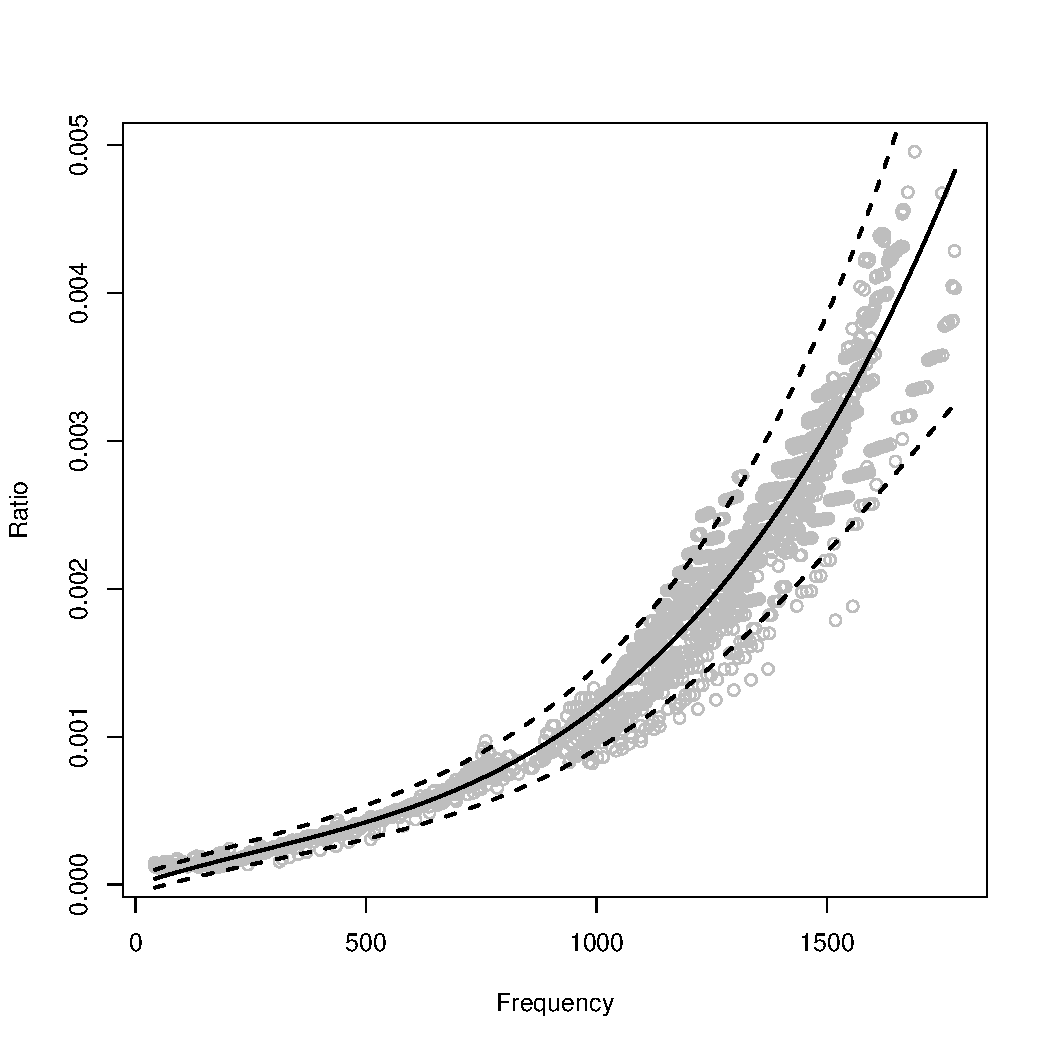
\includegraphics[width=0.5\textwidth]{plots/model}
 \caption{Ratio $M_{\rm PNS}/R_{\rm PNS}^2$ from 25 1D simulations {\sc AENUS-ALCAR} (red) and {\sc CoCoNuT} (green) code. The solid line is the maximum likelihood estimate of heteroscedastic cubic model with 95\% confidence bands (dashed lines) considering the {\sc AENUS-ALCAR} data points.} \label{fig:LMVAR}
\end{figure}

To develop the method we considered the gravitational wave signal
{\texttt s20S} described in Section \ref{sec:simulations}, originally
sampled at 16384 Hz but resampled at 4096 Hz.
A spectrogram of this signal is shown in Figure \ref{fig:spectrogram} based on
autoregressive estimates of the local spectra for successive time intervals of 
\textcolor{red}{length 200} with a \textcolor{red}{ 90\%} overlap.
The dominant emission mode corresponds to the PNS oscillation $\mbox{}^2 g_2$-mode. We have
developed a time-frequency method to track the ridge $m(t)$ in the spectrogram,
taking into account that it is monotonically increasing as time goes,
a property of the $\mbox{}^2 g_2$-mode.
Starting from either the left- or right-most column of the time-frequency matrix
we identify and trace the sequence of amplitude peaks within a certain frequency
band given the monotonicity constraint. Appendix \ref{app:gmode} is providing more
details on the reconstruction of the $g$ mode ridge. 


\begin{figure}
 \centering
 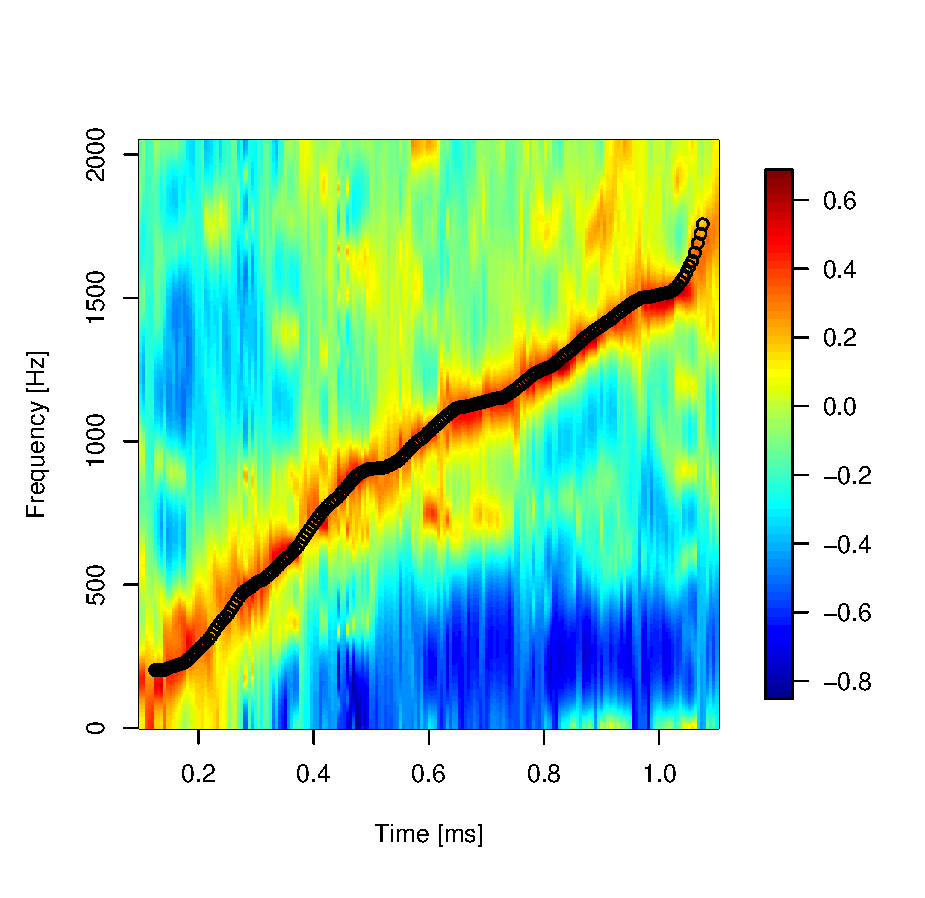
\includegraphics[width=0.5\textwidth]{plots/spectrogram}
 \caption{Spectrogram of the gravitational wave signal {\texttt s20S} sampled at \unit[4096]{Hz}.
   The spectrogram is obtained using data streach of 200 samples overlapping at 90\%
   with each other.} \label{fig:spectrogram}
\end{figure}


We collect the instantaneous frequency $f(t_i)$ corresponding to the ridge $m(t_i)$ for
the midpoint $t_i$ of each local time interval of the spectrogram and interpolating $f(t)$
for values in between the $t_i$. We then use equation \eqref{eq:model1} to obtain
estimates of the time evolution of the ratio together with 95\% confidence intervals.
An exemple is given in Figure \ref{fig:ratio} where the red points are the point estimates and
the grey bands represent 95\% confidence bands. Ratio values
computed using the mass and radius values obtained from the simulation code are shown in black.

\begin{figure}
 \centering
 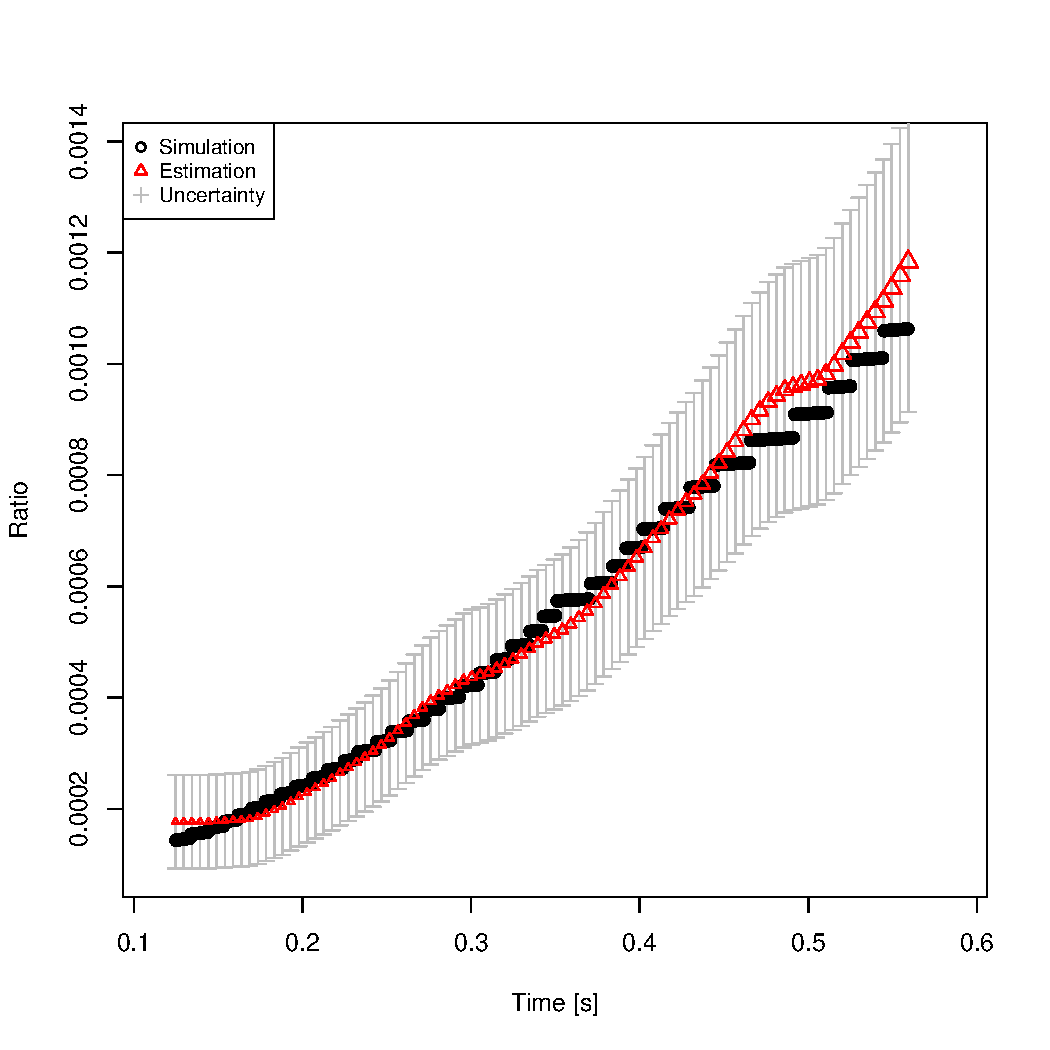
\includegraphics[width=0.5\textwidth,height=0.3\textheight]{plots/ratio}
 \caption{Ratio $M_{\rm PNS}/R_{\rm PNS}^2$ as function of time extracted from the $\mbox{}^2 g_2$-mode of the {\texttt s20S} signal (red points and the 95\% confidence belt in grey) compared to the ratio value derived from the PNS mass and radius given by the simulation code (black points).} \label{fig:ratio}
\end{figure}


In this case, for a GW signal without any noise, the coverage of our 95\% confidence band is 94\%.
In the next section we investigate the performance of reconstruction of $r(t)$ when the gravitational wave
signal is embedded in noise.
\bigskip

\section{Detection sensitivity with Advanced gravitational wave detectors}
\label{sec:results}

To estimate how accurately we can infer the time evolution of $r=M_{\rm PNS}/R_{\rm PNS}^2$ in the
gravitational wave detector data, we have added the {\tt s20-gw-10kpc} GW signal to hundred
Gaussian noise realisations whose power spectral density follows advanced LIGO
spectrum~\cite{aLIGOspectrum}. We have varied the distances to the source, covering a large
range of distances for which a detection is feasible. The source is optimally oriented with
respect to the gravitational wave detector. We are assuming a GW signal from a core collapse
phenomena has been identified in the data and that the beginning of the GW signal is known.
For each of the simulations, we reconstruct the ratio and compute few quantities that measure
the reconstruction accuracy. The first quantity is the coverage probability which is the
fraction of the ratio that falls within the 95\% confiddence interval.  


For that purpose, we inject the gravitational wave signal into  simulated Advanced LIGO noise
using the noise power spectral density \textcolor{red}{insert formula} for varying
SNRs, respectively distances to the source. We estimate the coverage probability of the 95\%
confidence band by calculating the proportion of times that the true ratio lies outside one
of the pointwise 95\% confidence intervals.
These coverage probabilities together for varying SNRs are given in Table
\textcolor{red}{insert Table} and displayed in the form of boxplots in Figure
\textcolor{red}{insert Figure}
\bigskip

\section{discussion}
\bigskip


\bigskip\noindent\textit{Acknowledgments} ---

\begin{appendices}
\section{G-mode reconstruction}
\label{app:gmode}
Given the spectrogram and an specified time interval for the g-mode reconstruction, our proposal method works as follows.  The starting point must be specified.  It can be either at the beginning or at the end of the signal.  Then, in one of these extremes, the maximum energy value is identified, registering its frequency.  This is done independently for a number of consecutive time intervals.  Then we calculate the median of these frequency values, providing a robust starting value for the g-mode reconstruction.

The starting frequency value is the first g-mode estimate for the first or the last time interval, depending on the specified starting location.  If the reconstruction is set to start at the beginning of the signal, the reconstruction will be done progressively over the time intervals, where each maximum frequency value will be calculated within a frequency range specified by the previous g-mode estimate.  Given the non-decreasing behaviour of the true g-mode values, the g-mode estimates will be forced to be greater or equal than the one estimated for its previous time interval, and lower than a specified upper limit.  As a result, the g-modes estimates will be a non-decreasing sequence of frequency values. 

If the reconstruction is set to start at the end of the signal, the g-modes will be estimated backward in time.  Each maximum frequency is calculated within a range determined by its successor (in time) g-mode estimate.  These estimates are forced to be lower or equal than its successor (in time) estimate, but greater than a specified lower limit. Thus, a non-decreasing sequence of g-mode estimates is guaranteed.

This g-mode reconstruction method works if and only if the signal is strong enough to provide information about the g-mode, which is reflected in the spectrogram.


Given the sequence of g-mode estimates, the confidence band will be calculated by using the model defined in \eqref{eq:universal}. The g-mode estimates are frequency values which we use as predictors in the model in order to generate confidence intervals for the ratios. Since the g-mode estimates are indexed by time, the confidence intervals for the ratios are too.  Thus, we generate the confidence band by interpolating the lower and upper limits of the collection of consecutive confidence intervals, which will be valid for the time range of the g-mode estimates.  This confidence band is used to estimate the coverage probabilities in our simulation studies presented below.  

\end{appendices}
%\bibliographystyle{unsrt}
\bibliography{biblio}


\end{document}
